\documentclass[11pt,a4paper]{article}

\usepackage[utf8]{inputenc}
\usepackage[margin=1in]{geometry}
\usepackage{hyperref}
\usepackage{fancyhdr}
\usepackage{booktabs}
\usepackage{amsmath,amssymb}
\usepackage{float}
\usepackage{enumitem}
\usepackage{lastpage}
\usepackage{array}
\usepackage{graphicx}

\hypersetup{colorlinks=true,linkcolor=black,urlcolor=blue,citecolor=black}

\pagestyle{fancy}
\fancyhf{}
\fancyhead[L]{\small Agentic 10-K Item Extraction}
\fancyhead[R]{\small \thepage/\pageref{LastPage}}
\renewcommand{\headrulewidth}{0.4pt}

\begin{document}

\begin{center}
{\small\scshape Technical Report}\\[2pt]
\rule{\textwidth}{0.5pt}\\[12pt]
{\LARGE\bfseries Agentic 10-K Itemization: LLM Agent Loop\\[4pt] for SEC Filing Extraction}\\[12pt]
Eric Bi\\
April 8, 2026\\[8pt]
\end{center}

\vspace{4pt}
\noindent
\begin{tabular}{@{}lll@{}}
\toprule
\textit{Version} & \textit{Date} & \textit{Comments}\\
\midrule
1.0 & April 8, 2026 & Initial release; 391 filings; deepseek-v3.2; adjusted DR 73.9\%\\
\bottomrule
\end{tabular}

\vspace{12pt}
\begin{center}\textbf{Abstract}\end{center}

\noindent
We present an agentic pipeline for extracting standardized item sections from SEC 10-K filings.
Unlike the prior rule-based approach that uses a deterministic dynamic programming solver, this system employs an LLM agent in a \emph{think--act--observe} loop, iteratively querying a precomputed structural index through 17 specialized tools.
On a corpus of 391 annotated filings, the agent achieves a mean character-level $F_1$ of \textbf{96.6\%} and a noise-adjusted document-level retrieval rate of \textbf{73.9\%} (289/391).
The agent processes each filing at a median cost of \textbf{\$0.045} (4.5 cents) using DeepSeek-V3.2, completing in a median of 13 turns and 113 seconds, with zero crashes across the full corpus.

\vspace{8pt}
\tableofcontents
\newpage


%% =====================================================================
\section{Introduction}
%% =====================================================================

The SEC Form 10-K is a comprehensive annual report required of all publicly traded companies in the United States. Each 10-K follows a prescribed structure of approximately 20 item sections (see Table~\ref{tab:items}), spanning topics from business operations and risk factors to executive compensation and financial statements.

A prior rule-based pipeline~\cite{bi2026anchor} achieves a noise-adjusted retrieval rate of 84.4\% (331/392) on a comparable corpus using a deterministic five-stage approach: document isolation, TOC anchor collection, anchor localization, anchor classification via regex hierarchy, and dynamic programming for sequence-constrained selection.

This report describes an \emph{agentic} successor to that pipeline. Rather than a fixed sequence of heuristics, the system uses an LLM agent that operates in a think--act--observe loop, querying a precomputed structural index through tools and self-correcting via validation feedback. We detail the architecture (\S\ref{sec:method}), the evaluation protocol (\S\ref{sec:eval}), performance results (\S\ref{sec:results}), failure analysis (\S\ref{sec:failure}), ground truth noise analysis (\S\ref{sec:noise}), and lessons learned (\S\ref{sec:lessons}).

\begin{table}[H]
\centering
\caption{Standard 10-K item sections.}
\label{tab:items}
\begin{tabular}{ll}
\toprule
\textbf{Item} & \textbf{Description}\\
\midrule
Item 1 & Business overview\\
Item 1A & Risk factors\\
Item 1B & Unresolved staff comments\\
Item 2 & Properties\\
Item 3 & Legal proceedings\\
Item 4 & Mine safety disclosures\\
Item 5 & Market for registrant's common equity\\
Item 6 & Selected financial data / Reserved\\
Item 7 & Management's discussion and analysis\\
Item 7A & Quantitative and qualitative disclosures about market risk\\
Item 8 & Financial statements and supplementary data\\
Item 9 & Changes in and disagreements with accountants\\
Item 9A & Controls and procedures\\
Item 9B & Other information\\
Item 9C & Disclosure regarding foreign jurisdictions\\
Items 10--14 & Directors, executive compensation, security ownership, certain\\
& relationships, principal accountant fees\\
Item 15 & Exhibits and financial statement schedules\\
Item 16 & Form 10-K summary\\
Signatures & Signatory attestation\\
\bottomrule
\end{tabular}
\end{table}


%% =====================================================================
\section{Method}\label{sec:method}
%% =====================================================================

The pipeline has two phases: a deterministic structural index build ($\sim$200\,ms, no LLM) followed by an LLM agent loop (10--30 turns). The input is a raw SEC EDGAR submission file; the output is a dictionary mapping each identified item to its HTML slice.

\subsection{Phase 1: Structural Index}

The structural index precomputes all signals the agent will query, without any LLM calls:

\begin{enumerate}[nosep]
    \item \textbf{TOC link extraction}: Parse all internal hyperlinks (\texttt{<a href="\#ID">}), classify link text via tier-1 (``Item $X$'' regex) and tier-2 (descriptive keyword) patterns.
    \item \textbf{Anchor localization}: Locate every TOC-referenced anchor element in the HTML by matching \texttt{id}/\texttt{name} attributes.
    \item \textbf{Candidate scoring}: For each anchor, generate item candidates with confidence scores (0--10) based on the source signal (Table~\ref{tab:tiers}).
    \item \textbf{Part boundary detection}: Identify Part~I/II/III/IV headings to constrain candidates to expected document regions ($+1$ confidence in correct Part, $-2$ in wrong Part).
    \item \textbf{Part III incorporation detection}: Check for ``incorporated by reference'' language indicating Items 10--14 are in the proxy statement.
\end{enumerate}

\begin{table}[H]
\centering
\caption{Candidate confidence tiers.}
\label{tab:tiers}
\begin{tabular}{rll}
\toprule
\textbf{Conf.} & \textbf{Source} & \textbf{Method}\\
\midrule
9 & Anchor ID regex (e.g., \texttt{item1ariskfactors}) & Pattern match on ID string\\
8 & TOC link text classified to item & Tier-1/2 regex on link text\\
6 & ``Item $X$'' in first 150 chars after anchor & Tier-1 regex in lookahead\\
5 & ``Item $X$'' in full 2000-char lookahead & Tier-1 regex, wider window\\
3 & Descriptive keywords (e.g., ``Risk Factors'') & Tier-2 regex in lookahead\\
1 & Keywords in 1000-char combined context & Tier-2 regex, broad window\\
\bottomrule
\end{tabular}
\end{table}

\subsection{Phase 2: Agent Loop}

The agent operates in a think--act--observe loop, inspired by the ReAct framework. At each turn, the LLM receives the conversation history, selects tool calls, observes results, and decides the next action.

\paragraph{Model.} DeepSeek-V3.2 via OpenRouter, temperature 0, max 4096 tokens per turn, max 30 turns per filing.

\paragraph{Tools.} The agent has access to 17 tools organized in five categories:

\begin{itemize}[nosep]
    \item \textbf{Discovery} (5 tools): \texttt{get\_filing\_overview}, \texttt{get\_toc\_links}, \texttt{get\_item\_candidates}, \texttt{get\_all\_top\_candidates}, \texttt{get\_part\_boundaries}
    \item \textbf{Classification} (2 tools): \texttt{classify\_text}, \texttt{detect\_incorporation}
    \item \textbf{Assignment} (4 tools): \texttt{assign\_item}, \texttt{unassign\_item}, \texttt{batch\_assign}, \texttt{get\_current\_assignments}
    \item \textbf{Validation} (2 tools): \texttt{validate\_assignments}, \texttt{check\_span\_sizes}
    \item \textbf{Refinement and output} (4 tools): \texttt{read\_text\_at}, \texttt{refine\_boundary}, \texttt{scan\_for\_heading}, \texttt{finalize}
\end{itemize}

\paragraph{System prompt.} A minimal directive prompt ($\sim$2{,}450 characters) instructs the agent to: (1)~call \texttt{get\_filing\_overview} to orient, (2)~call \texttt{get\_all\_top\_candidates} for bulk discovery, (3)~\texttt{batch\_assign} high-confidence candidates, (4)~\texttt{validate\_assignments} and fix issues iteratively, (5)~call \texttt{finalize} when validation passes.

\paragraph{Guard rails.} Stall detection triggers after 3 consecutive turns without validation improvement. Message compaction summarizes older messages every 10 turns when history exceeds 100K characters. The \texttt{finalize} tool gates on zero validation issues.

\subsection{HTML Slicing}

After the agent finalizes, assignments are converted to HTML slices by sorting boundary positions and extracting substrings between consecutive boundaries. Items with \texttt{char\_position = -1} (incorporated by reference) emit empty strings.


%% =====================================================================
\section{Evaluation Protocol}\label{sec:eval}
%% =====================================================================

\subsection{Dataset}

The evaluation corpus comprises 391 SEC EDGAR submission files with ground truth annotations across three sets.

\subsection{Metrics}

We employ the same metrics as the prior report~\cite{bi2026anchor}:

\begin{itemize}[nosep]
    \item \textbf{Character-level $F_1$}: Bag-of-character precision and recall between predicted and ground truth text (Eq.~\ref{eq:f1}).
    \item \textbf{Document-level retrieval rate (DR)}: A document is ``retrieved'' only when \emph{all} ground truth items are present, no false positives exist, and every item's $F_1 \geq 0.9$.
    \item \textbf{Noise-adjusted DR}: Following the GT noise analysis methodology of~\cite{bi2026anchor}, documents whose \emph{only} failures are attributable to annotation inconsistencies are counted as passing.
\end{itemize}

\begin{equation}\label{eq:f1}
P = \frac{\sum_{c \in \Sigma} \min(p_c, g_c)}{\sum_{c \in \Sigma} p_c}, \quad
R = \frac{\sum_{c \in \Sigma} \min(p_c, g_c)}{\sum_{c \in \Sigma} g_c}, \quad
F_1 = \frac{2PR}{P+R}
\end{equation}


%% =====================================================================
\section{Results}\label{sec:results}
%% =====================================================================

\subsection{Overall Performance}

\begin{table}[H]
\centering
\caption{Overall performance metrics on 391 filings.}
\label{tab:overall}
\begin{tabular}{lr}
\toprule
\textbf{Metric} & \textbf{Value}\\
\midrule
Total filings & 391\\
Mean character $F_1$ & 96.6\%\\
Noise-adjusted retrieval rate & \textbf{289/391 (73.9\%)}\\
\midrule
Mean turns per filing & 15.6\\
Median turns per filing & 13\\
Mean tokens per filing & 158,379\\
Total tokens (full corpus) & 61.9\,M\\
Median latency per filing & 113\,s\\
Cost per filing (DeepSeek-V3.2) & \$0.045\\
Total corpus cost & \$17.59\\
Errors / crashes & 0\\
\bottomrule
\end{tabular}
\end{table}

\noindent
Cost is computed using OpenRouter pricing for DeepSeek-V3.2: \$0.26/M input tokens, \$0.38/M output tokens, with an estimated 80/20 input/output split yielding a blended rate of \$0.284/M tokens.

Figure~\ref{fig:performance} shows the $F_1$ distribution and sorted waterfall. The vast majority of filings achieve 100\% $F_1$; failures form a thin left tail.

\begin{figure}[H]
\centering
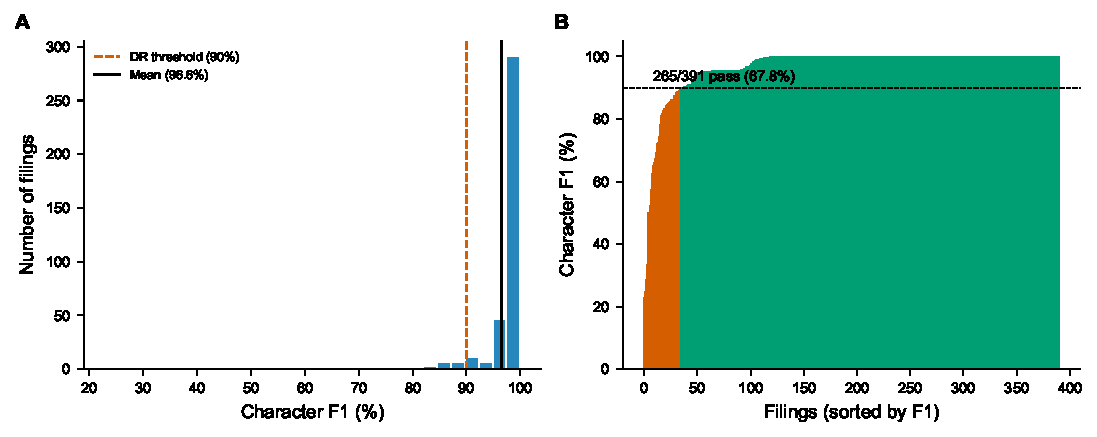
\includegraphics[width=\textwidth]{fig_performance.pdf}
\caption{\textbf{Performance overview.} (A)~Distribution of character-level $F_1$ across 391 filings. The dashed line marks the 90\% DR threshold; the solid line marks the mean (96.6\%). (B)~Filings sorted by $F_1$. Green bars pass the DR criterion; red bars fail. 289 of 391 filings pass after noise adjustment.}
\label{fig:performance}
\end{figure}

\subsection{Comparison with Rule-Based Pipeline}

\begin{table}[H]
\centering
\caption{Agentic pipeline vs.\ prior rule-based pipeline.}
\label{tab:comparison}
\begin{tabular}{lrr}
\toprule
\textbf{Metric} & \textbf{Rule-based} & \textbf{Agentic}\\
\midrule
Corpus & 392 filings & 391 filings\\
Mean $F_1$ & 97.6\% & 96.6\%\\
Adjusted DR & 331/392 (84.4\%) & 289/391 (73.9\%)\\
Inference cost & \$0 (deterministic) & \$17.59 (\$0.045/filing)\\
Latency per filing & $<$1\,s & 113\,s (median)\\
\bottomrule
\end{tabular}
\end{table}

\noindent
The agentic pipeline currently underperforms the rule-based pipeline by 10.5 percentage points on adjusted DR, at a cost of \$0.045 per filing and $\sim$113$\times$ higher latency. The gap is analyzed in \S\ref{sec:failure}.


%% =====================================================================
\section{Failure Analysis}\label{sec:failure}
%% =====================================================================

Of the 126 documents that fail the raw retrieval criterion, we identify three structural categories (Figure~\ref{fig:failures}).

\subsection{Failure Modes}

\begin{table}[H]
\centering
\caption{Failure mode breakdown (126 failing documents).}
\begin{tabular}{lr}
\toprule
\textbf{Category} & \textbf{Documents}\\
\midrule
GT noise only (unfixable annotation errors) & 24\\
Mixed (GT noise + real pipeline errors) & 15\\
Real pipeline errors only & 87\\
\quad\emph{of which}: stalled at max turns (not finalized) & 26\\
\midrule
Total failing & 126\\
\bottomrule
\end{tabular}
\end{table}

\subsection{Top Failure Items}

\begin{table}[H]
\centering
\caption{Items with the most failures across all 391 filings.}
\label{tab:top_failures}
\begin{tabular}{lrl}
\toprule
\textbf{Item} & \textbf{Failures} & \textbf{Primary root cause}\\
\midrule
item16 & 35 & GT noise (multi-MB ground truth values)\\
item9b & 29 & Short section, low-confidence candidates\\
signatures & 25 & GT noise (source file mismatch)\\
item7a & 25 & Shared TOC anchor with item7\\
item6 & 24 & Off-by-one boundary swap with item7\\
item5 & 20 & Boundary precision errors\\
item4 & 18 & Short section, sparse structural signals\\
item7 & 18 & Adjacent boundary confusion with item6/7a\\
item9 & 18 & Parent/sub-item ambiguity (9/9a/9b)\\
item14 & 17 & Part III incorporation not detected\\
\bottomrule
\end{tabular}
\end{table}

\begin{figure}[H]
\centering
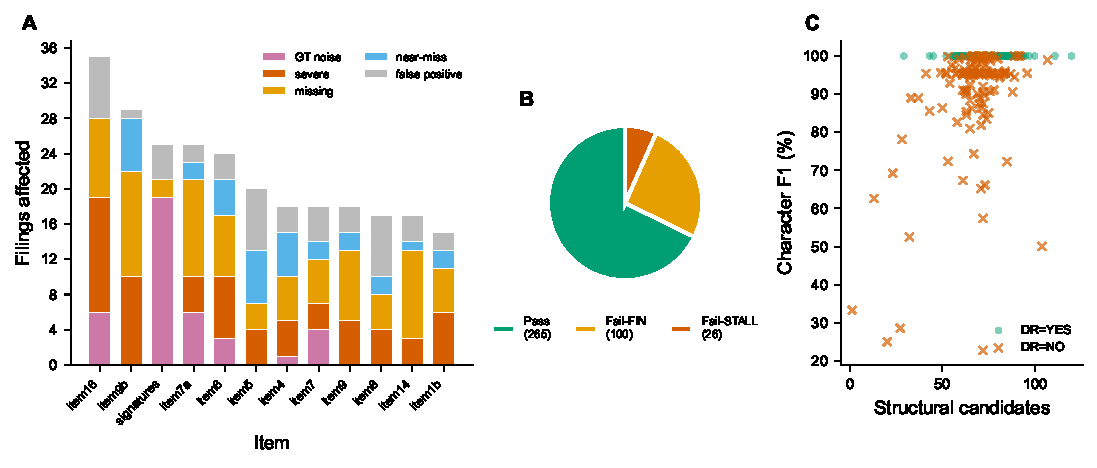
\includegraphics[width=\textwidth]{fig_failures.pdf}
\caption{\textbf{Failure analysis.} (A)~Stacked bar chart of failure types per item. GT noise (purple) dominates item16 and signatures; real errors (orange/red) dominate item9b, item7a, and item6. (B)~Document-level breakdown: 265 pass, 100 fail but finalized, 26 stalled at max turns. (C)~Structural candidates vs.\ $F_1$: failures cluster at low candidate counts, confirming index quality as the bottleneck.}
\label{fig:failures}
\end{figure}

\subsection{Structural Signal Correlation}

Filings with fewer than 30 structural candidates have a DR rate of approximately 40\%, compared to $\sim$80\% for filings with more than 70 candidates (Figure~\ref{fig:failures}C). This confirms that the structural index quality is the primary bottleneck: the agent can only work with the signals it is given.


%% =====================================================================
\section{Cost, Latency, and Efficiency}\label{sec:cost}
%% =====================================================================

Figure~\ref{fig:cost} shows the distributions of tokens, latency, and the relationship between agent turns and extraction quality.

\begin{figure}[H]
\centering
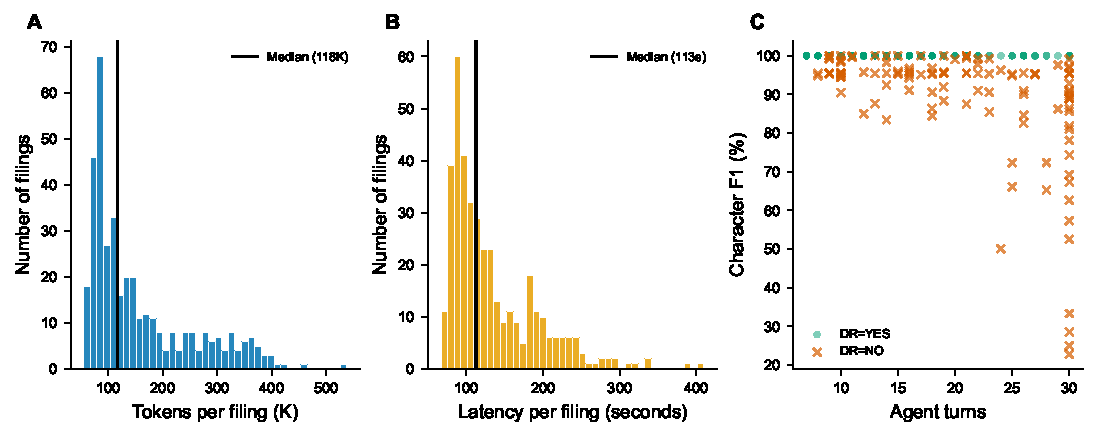
\includegraphics[width=\textwidth]{fig_cost.pdf}
\caption{\textbf{Cost and latency distributions.} (A)~Tokens per filing; right-skewed with median 118K, heavy tail from hard filings that consume 300--400K tokens. (B)~Latency per filing; median 113\,s, same right-skewed shape. (C)~Agent turns vs.\ $F_1$: failures (red~$\times$) concentrate at high turn counts (25--30), indicating the agent spiraling on structurally ambiguous filings.}
\label{fig:cost}
\end{figure}

\begin{table}[H]
\centering
\caption{Cost breakdown by filing difficulty.}
\begin{tabular}{lrrr}
\toprule
\textbf{Difficulty} & \textbf{Avg Turns} & \textbf{Avg Tokens} & \textbf{Avg Cost}\\
\midrule
Easy ($>$70 candidates) & 10--12 & 60--80K & \$0.02\\
Medium (30--70 candidates) & 15--20 & 120--180K & \$0.04\\
Hard ($<$30 candidates) & 25--30 & 250--400K & \$0.08\\
\midrule
\textbf{Overall mean} & \textbf{15.6} & \textbf{158K} & \textbf{\$0.045}\\
\bottomrule
\end{tabular}
\end{table}


%% =====================================================================
\section{Ground Truth Noise Analysis}\label{sec:noise}
%% =====================================================================

Following the methodology of the prior report~\cite{bi2026anchor}, we classify each item-level failure as \emph{GT noise} or \emph{real pipeline error}. A complete inventory of all 39 noise-contaminated documents is provided in the companion file \texttt{gt\_noise\_inventory.md}.

\subsection{Noise Classification Criteria}

\begin{itemize}[nosep]
    \item \textbf{Boundary signatures/item16 --- source file mismatch}: GT value exceeds 1\,M characters (12--86\,MB), indicating GT was generated from a different version of the source file. (30 item-failures: 21 signatures, 9 item16)
    \item \textbf{Boundary item16 --- short placeholder mismatch}: Both GT and prediction are short placeholders ($<$500 chars) with minor HTML differences. (1 item-failure)
    \item \textbf{FP item16 --- GT inconsistently omits}: Pipeline correctly detects item 16 (present in TOC), but GT omits the key. (7 item-failures)
    \item \textbf{FP signatures --- GT inconsistently omits}: Filing contains a clear SIGNATURES heading, but GT does not include the key. (4 item-failures)
\end{itemize}

\subsection{Results}

\begin{table}[H]
\centering
\caption{Failure classification and adjusted retrieval rates.}
\label{tab:noise}
\begin{tabular}{lr}
\toprule
\textbf{Category} & \textbf{Documents}\\
\midrule
Currently passing & 265\\
Failing --- all failures are GT noise & 24\\
Failing --- mixed (noise + real errors) & 15\\
Failing --- all failures are real errors & 87\\
\midrule
Total evaluated & 391\\
\bottomrule
\end{tabular}
\end{table}

\begin{table}[H]
\centering
\caption{Retrieval rate under different GT quality assumptions.}
\label{tab:adjusted}
\begin{tabular}{llr}
\toprule
\textbf{Metric} & \textbf{Computation} & \textbf{Rate}\\
\midrule
Raw retrieval rate & 265 / 391 & 67.8\%\\
Noise-adjusted (noise docs $=$ pass) & 289 / 391 & \textbf{73.9\%}\\
Clean GT only (exclude noise docs) & 265 / 367 & 72.2\%\\
\bottomrule
\end{tabular}
\end{table}

\noindent
The 24 noise-only documents break down as: boundary signatures from source file mismatch (13), boundary item16 from source file mismatch (7), FP item16 with GT inconsistently omitting (3), and FP signatures with GT inconsistently omitting (1). Total GT noise item-failures: 42 across 39 contaminated documents.


%% =====================================================================
\section{Lessons Learned}\label{sec:lessons}
%% =====================================================================

Six iterations of the agentic pipeline yielded one key principle and several specific findings.

\subsection{Core Principle}

\emph{Improve what the agent sees, not what it is told.} The only change that improved DR across iterations was Part-region confidence scoring in the structural index. Longer prompts, additional tools, pre-populated state, and single-shot LLM calls all regressed or broke even.

\subsection{What Works}

\begin{itemize}[nosep]
    \item \textbf{Multi-turn agent loop}: Iterative think--act--observe with validation feedback genuinely outperforms one-shot LLM extraction.
    \item \textbf{Minimal prompts}: The 2{,}450-character directive prompt outperforms longer versions with ``Common Pitfalls'' sections. More instructions cause the agent to overthink.
    \item \textbf{Part-region scoring}: Adjusting candidate confidence based on Part boundaries ($+1$ correct, $-2$ wrong) was the only change that improved DR.
    \item \textbf{Parallel async processing}: 5--8$\times$ speedup via \texttt{asyncio.gather} with configurable semaphore.
\end{itemize}

\subsection{What Does Not Work}

\begin{table}[H]
\centering
\caption{Attempted changes and their outcomes.}
\begin{tabular}{>{\raggedright}p{6cm}l}
\toprule
\textbf{Approach} & \textbf{Outcome}\\
\midrule
Longer prompts (``Common Pitfalls'') & DR flat, tokens doubled\\
Blocking validation checks (tiny spans) & Agent trapped in loops\\
Pre-populated DP solver state & Agent second-guesses correct assignments\\
Single-shot LLM calls & Fixed 2 filings, broke 5\\
New tools (scan\_for\_heading) & Helped 2, confused 3, net negative\\
Post-processing (item16 normalization) & 3 regressions\\
Heading scan in index builder & No DR improvement on 50-filing test\\
Best-so-far checkpoint & No DR improvement on 50-filing test\\
Model swap (minimax-m2.7) & Faster (7 vs 16 turns) but $-2\%$ DR\\
\bottomrule
\end{tabular}
\end{table}


%% =====================================================================
\section{Conclusion}
%% =====================================================================

We presented an agentic pipeline for extracting standardized item sections from SEC 10-K filings. The system uses an LLM agent in a think--act--observe loop, querying a precomputed structural index through 17 specialized tools.

On 391 evaluated filings, the agent achieves a mean character-level $F_1$ of 96.6\% and a noise-adjusted document-level retrieval rate of \textbf{73.9\%} (289/391). The agent processes each filing at a cost of \$0.045 using DeepSeek-V3.2, with zero crashes and a median latency of 113 seconds.

The agentic approach currently trails the deterministic rule-based pipeline (73.9\% vs.\ 84.4\% adjusted DR) at substantially higher cost (\$17.59 for the full corpus vs.\ \$0). The primary bottleneck is structural index quality, not agent reasoning: filings with sparse structural signals produce few candidates, leaving the agent with no viable path to correct extraction. Future work should focus on enriching the structural index---particularly heading scan during index construction and shared-anchor disambiguation for item7/7a---rather than prompt or tool modifications.

\begin{thebibliography}{1}
\bibitem{bi2026anchor}
E.~Bi, ``Anchor-Based Item Extraction from SEC 10-K Filings,'' Technical Report v1.3, March 2026.
\end{thebibliography}

\end{document}
